\themaM
\graphicspath{{../Ch26_Volumes_et_capacites/Images/}}

\chapter{Volumes et\\contenances}
\label{C19}


%%%%%%%%%%%%%%%%%%%%%%%%%%%%%%%%%%%%%%%%%%
\begin{prerequis}[Connaissances et compétences abordées]
   \begin{itemize}
      \item Connaître le lien entre les unités de numération et les unités de mesure (par exemple : dixième -> dL, centième -> cL).
      \item Relier les unités de volume et de contenance.
      \item  Estimer la mesure d’un volume ou d’une contenance par différentes procédures (transvasements, appréciation de l’ordre de grandeur) et l’exprimer dans une unité adaptée.
      \item Unités usuelles de contenance (multiples et sous multiples du litre) ; unités usuelles de volume (cm$^3$ , dm$^3$ , m$^3$), relations entre ces unités.
   \end{itemize}
\end{prerequis}

\vfill

\begin{debat}[Débat : 1 L = 1 \udmc{}]
   Cette correspondance est à connaître. Pourtant, elle ne paraît pas si naturelle que cela : elle signifie que l'eau contenue dans une bouteille d'un litre remplirait exactement un cube de \udm{1} de côté.
   \begin{center}
      \begin{pspicture}(0,-0.25)(6,5.5)
         \psline(0.5,0.5)(0.5,3.75) %bouteille
         \psline(2,0.5)(2,3.75)
         \psarc(1.5,3.75){0.5}{0}{90}
         \psarc(1,3.75){0.5}{90}{180}
         \psline(1,4.25)(1,5)
         \psline(1.5,4.25)(1.5,5)
         \psellipticarc(1.25,0.5)(0.75,0.3){180}{0}
         \psellipticarc(1.25,3.5)(0.75,0.3){180}{0}
         \psellipticarc[linestyle=dashed](1.25,3.5)(0.75,0.3){0}{180}
         \psellipse(1.25,5)(0.25,0.1)
         \rput(1.25,2){\textcolor{B1}{\ul{1}}}
         \psframe(3,0.5)(5,2.5) %cube
         \psline(3,2.5)(3.75,3.25)(5.75,3.25)(5.75,1.25)(5,0.5)
         \psline(5,2.5)(5.75,3.25)
         \rput(4,0.2){\textcolor{B1}{$\udm{1} =\ucm{10}$}}
         \rput(4,1.5){\textcolor{B1}{$\udmc{1}$}}
      \end{pspicture}
   \end{center}
   \bigskip
   \begin{cadre}[B2][F4]
      \begin{center}
         Vidéo : \href{https://www.youtube.com/watch?v=DRKmlWtUN0k}{\bf Correspondance entre unités de volume et de contenance}, chaîne YouTube de {\it Jean-Charles Toussaint}.
      \end{center}
   \end{cadre}
\end{debat}

\vfill

\textcolor{PartieGeometrie}{\sffamily\bfseries Cahier de compétences} : chapitre 12, exercices 12 ; 15 à 17 ; 20 à 24.


%%%%%%%%%%%%%%%%%%%%%%%%%%%%%%%
%%%%%%%%%%%%%%%%%%%%%%%%%%%%%%%
\activites

\begin{activite}[Des petits cubes]
   {\bf Objectifs :} déterminer le volume d'un solide par dénombrement ; analyser un solide en trois dimensions.
   \begin{QCM}
      \partie[des cubes de cubes]
         Donner le nombre de petits cubes qui composent chacun des solides suivants : \\
         \begin{center}
            \includegraphics[width=15cm]{cube} \\ [10mm]
         \end{center}
         
      \partie[à vous de jouer !]
         Dessiner trois solides différents comportant huit petits cubes chacun.
         \begin{center}
            {\psset{unit=0.5}
            \begin{pspicture}(0,-0.5)(30,10.5)
               \psgrid[subgriddiv=1,gridlabels=0,gridcolor=lightgray](0,0)(30,10)
               \psframe(1,7)(2,8)
               \pspolygon[fillstyle=solid,fillcolor=lightgray](1,8)(1.5,8.5)(2.5,8.5)(2,8)
               \pspolygon[fillstyle=solid,fillcolor=gray](2.5,8.5)(2,8)(2,7)(2.5,7.5)
            \end{pspicture}}
         \end{center}
   \end{QCM}
\vfill\hfill{\it\footnotesize Source : \href{http://www-irem.univ-paris13.fr/site_spip/spip.php?article348}{IREM Paris-Nord}}
\end{activite}


%%%%%%%%%%%%%%%%%%%%%%%%%%%%%%%
%%%%%%%%%%%%%%%%%%%%%%%%%%%%%%%
\cours 

%%%%%%%%%%%%%%%%%%%%%%%%%%%%%%%
\section{Volume par dénombrement}

\begin{definition}
   Le \textbf{volume} est une grandeur physique qui mesure l'espace occupé par celui-ci.
\end{definition}

\begin{exemple*1}
   Ces trois objets n'ont pas la même forme mais occupent la même quantité d'espace.
   \begin{center}
      \begin{pspicture}(0,-1)(13,3.8)
         \psset{linecolor=A1}
         \psframe(0,0)(3,2)
         \psline(1,0)(1,2)(1.5,2.5)
         \psline(2,0)(2,2)(2.5,2.5)
         \psline(0,1)(3,1)(3.5,1.5)
         \psline(3,0)(3.5,0.5)(3.5,2.5)(0.5,2.5)(0,2)
         \psline(3,2)(3.5,2.5)  
         \psset{linecolor=B1}    
         \pspolygon(5,0)(9,0)(9,2)(8,2)(8,1)(6,1)(6,2)(5,2)
         \psline(5,1)(6,1)(6,0)
         \psline(7,0)(7,1)(7.5,1.5)
         \psline(9,0)(9.5,0.5)(9.5,2.5)(8.5,2.5)(8,2)
         \psline(9,2)(9.5,2.5)
         \psline(9.5,1.5)(9,1)(8,1)(8,0)
         \psline(5,2)(5.5,2.5)(6.5,2.5)(6.5,1.5)(8,1.5)
         \psline(6,2)(6.5,2.5)
         \psline(6,1)(6.5,1.5)     
         \psset{linecolor=G1} 
         \pspolygon(11,0)(14,0)(14,1)(13,1)(13,2)(12,2)(12,3)(11,3)
         \psline(12,0)(12,1)(11,1)
         \psline(13,0)(13,1)(12,1)(12,2)(11,2)
         \psline(14,0)(14.5,0.5)(14.5,1.5)(13.5,1.5)(13.5,2.5)(12.5,2.5)(12.5,3.5)(11.5,3.5)(11,3)
         \psline(14,1)(14.5,1.5)
         \psline(13,2)(13.5,2.5)
         \psline(12,3)(12.5,3.5)
         \psline(13,1)(13.5,1.5)
         \psline(12,2)(12.5,2.5)
      \end{pspicture}
   \end{center}
   Si l'unité de volume ({\it u.v.}) est ce cube \begin{pspicture}(-0.1,0.5)(1.6,1) \psline(0,1)(0,0)(1,0)(1,1)(0,1)(0.5,1.5)(1.5,1.5)(1.5,0.5)(1,0) \psline(1,1)(1.5,1.5) \end{pspicture}, le volume des trois solides est de 6 {\it u.v.} \\
\end{exemple*1}


%%%%%%%%%%%%%%%%%%%%%%%%%%%%%
\section{Unités de volume et de contenance}

\smallskip

Il existe deux unités principales de mesure en dimension 3 : les unités de volume en \og cube \fg{} et les unités de capacité en \og litre \fg. 

\begin{definition}
   \begin{itemize}
      \item Le {\bf mètre cube} (\umc{}) est une unité de volume qui correspond à un cube d'arête \um{1}.
      \item Le {\bf litre} (L) est une unité de capacité qui sert à exprimer la contenance d’un objet.
   \end{itemize}
\end{definition}

\bigskip
     $$\fbox{$\ul{1} = \udmc{1} \quad \text{et} \quad \ul{1000} =\umc{1}$}$$ 

Pour effectuer un changement d'unité de volume, on reprend les même préfixes que pour les changements de longueur, et on impose pour chacun d'eux trois colonnes au tableau.
\begin{center}
   {\hautab{1.2}
      \begin{ltableau}{0.9\linewidth}{21}
         \hline
         \multicolumn{3}{|c|}{\ukmc{}}
         & \multicolumn{3}{c|}{\uhmc{}}
         & \multicolumn{3}{c|}{\udamc{}}
         & \multicolumn{3}{c|}{\umc{}}
         & \multicolumn{3}{c|}{\udmc{}}
         & \multicolumn{3}{c|}{\ucmc{}}
         & \multicolumn{3}{c|}{\ummc{}} \\
         \hline
         & & & & & & & & & & & & \!hL & \!\!daL & L & \!dL & \!cL & \!\!mL & & & \\
         \hline
         & & & & & & & 2 & 1 & 0 & 9 & 2 & 8 & 0 & 1 & 5 & & & & & \\
         \hline
      \end{ltableau}}
\end{center}

\smallskip

Ainsi, pour convertir d'une unité à l'autre; on multiplie ou on divise par \numprint{1000}, \numprint{1000000}\dots

\begin{exemple*1}
    \umc{21092,8015} = \udamc{21,0928015} \\
    \hspace*{4cm} = \udmc{21092801,5} =\ul{21092801,5} \\
    \hspace*{4cm} = \ucmc{21092801500} =\uml{21092801500} \\
    \hspace*{4cm} = \ummc{21092801500000}
\end{exemple*1}
   
   
%%%%%%%%%%%%%%%%%%%%%%%%%%%%
%%%%%%%%%%%%%%%%%%%%%%%%%%%%
\exercicesbase

\begin{colonne*exercice}

\serie{Conversions et associations} %%%%%

\begin{exercice}
   Effectuer les conversions de volumes suivantes : \medskip
   \begin{enumerate}
      \item \udmc{1} = \pfb \ummc{} \medskip
      \item \ummc{200} = \pfb \ucmc{} \medskip
      \item \ukmc{1542} = \pfb \udamc{} \medskip
      \item \ucmc{35,635} = \pfb \ummc{} \medskip
      \item \umc{534273} = \pfb \ukmc{} \medskip
   \end{enumerate}
\end{exercice}

\begin{exercice}
   Effectuer les conversions de capacités suivantes : \medskip
   \begin{enumerate}
      \item \ul{1} = \pfb \udl{} \medskip
      \item \udal{1,53} = \pfb \ucl{} \medskip
      \item \udl{35} = \pfb \ul{} \medskip
      \item \udl{12} = \pfb \udal{} \medskip
      \item \uml{172,4} = \pfb \udl{} \medskip
   \end{enumerate}
\end{exercice}

\begin{exercice}
   Effectuer les conversions volume/capacité suivantes : \medskip
   \begin{enumerate}
      \item \udmc{1} = \pfb \ul{} \medskip
      \item \umc{1} = \pfb \ul{} \medskip
      \item \uhl{1} = \pfb \ucmc{} \medskip
      \item \ul{131,2} = \pfb \umc{} \medskip
      \item \ucmc{35,635} = \pfb \udl{} \medskip
   \end{enumerate}
\end{exercice}

\begin{exercice}
   Associer à chaque volume ou capacité l'objet qui lui correspond. \\ [1mm]
   {\hautab{1.4}
   \begin{tabular}{|p{2cm}|C{1.8}|p{3cm}|}
      \cline{1-1} \cline{3-3}
      \hfill \ul{16} & $\bullet \hfill \bullet$ & Maison \\
      \cline{1-1} \cline{3-3}
      \hfill \uhmc{1} & $\bullet \hfill \bullet$ & Cartable \\
      \cline{1-1} \cline{3-3}
      \hfill \ummc{10} & $\bullet \hfill \bullet$ & Baignoire \\
      \cline{1-1} \cline{3-3}
      \hfill \umc{600} & $\bullet \hfill \bullet$ & Mer méditerranée \\
      \cline{1-1} \cline{3-3}
      \ukmc{3700000} & $\bullet \hfill \bullet$ & Bille \\
      \cline{1-1} \cline{3-3}
      \hfill \ucmc{5} & $\bullet \hfill \bullet$ & {\small Empire State Building} \\
      \cline{1-1} \cline{3-3}
      \hfill \ul{200} & $\bullet \hfill \bullet$ & Grain de riz \\
      \cline{1-1} \cline{3-3}
   \end{tabular}}
\end{exercice}

\medskip

\serie{Calcul de volumes} %%%%%

\begin{exercice}
   Donner le volume de chaque solide en unités de volume (les solides sont supposés pleins).
   \begin{center}
      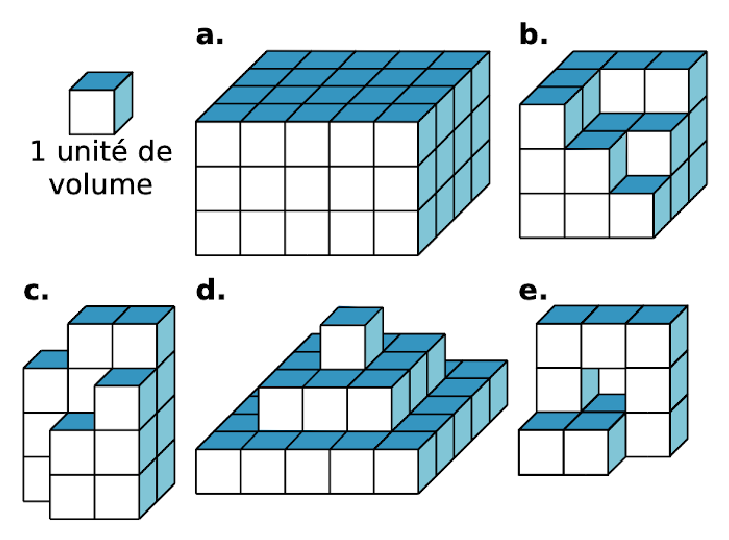
\includegraphics[width=8cm]{cubes}
   \end{center}
\end{exercice}



\hfill {\it\footnotesize Source : D’après Les cahiers Sésamath 6e. Magnard-Sesamath 2017}

\end{colonne*exercice}

\begin{center}
   {\bf Tableau d'aide à la conversion}
\end{center}
{\psset{unit=0.62}
   \begin{pspicture}(-0.5,10)(26,18.2)
      \multido{\r=0+1.25}{22}{\psline(\r,9)(\r,16)}
      \psset{linewidth=0.4mm}
      \multido{\r=0+3.75}{8}{\psline(\r,9)(\r,18)}
      \psline(0,18)(26.25,18)
      \psline(0,17)(26.25,17)
      \psline(0,16)(26.25,16)
      \rput(3,16.5){\bf km$^3$}
      \rput(6.8,16.5){\bf hm$^3$}
      \rput(10.4,16.5){\bf dam$^3$}
      \rput(14.3,16.5){\bf m$^3$}
      \rput(18,16.5){\bf dm$^3$}
      \rput(18.1,17.5){\bf L}
      \rput(19.4,17.5){\bf dL}
      \rput(20.6,17.5){\bf cL}
      \rput(21.9,17.5){\bf mL}
      \rput(16.9,17.5){\bf daL}
      \rput(15.6,17.5){\bf hL}
      \rput(21.7,16.5){\bf cm$^3$}
      \rput(25.5,16.5){\bf mm$^3$}
   \end{pspicture}}


%%%%%%%%%%%%%%%%%%%%%
%%%%%%%%%%%%%%%%%%%%%
\Recreation

\enigme[Visualiser pour calculer]
   \partie[Partie 1 - Accès à l'activité]
   
   Aller sur le site Internet de l'IREM de Paris-Nord : Rubricamaths, rubrique \og Visualiser pour calculer (1) \fg. \\
   Voilà son adresse : \href{www-irem.univ-paris13.fr/site_spip/spip.php?rubrique121}{\texttt{www-irem.univ-paris13.fr/site\_spip/spip.php?rubrique121}} \\
   
   \begin{tabular}{C{8}|C{8}}
      Choisir l'un des solides proposés dans la partie 2 en cliquant sur {\red\underline{En ligne}} & Pour chacun de ces solides, indiquer le volume en \og cubes \fg. Un résultat juste apparaitra sur fond vert, un résultat faux apparaitra sur fond rouge. \\ 
      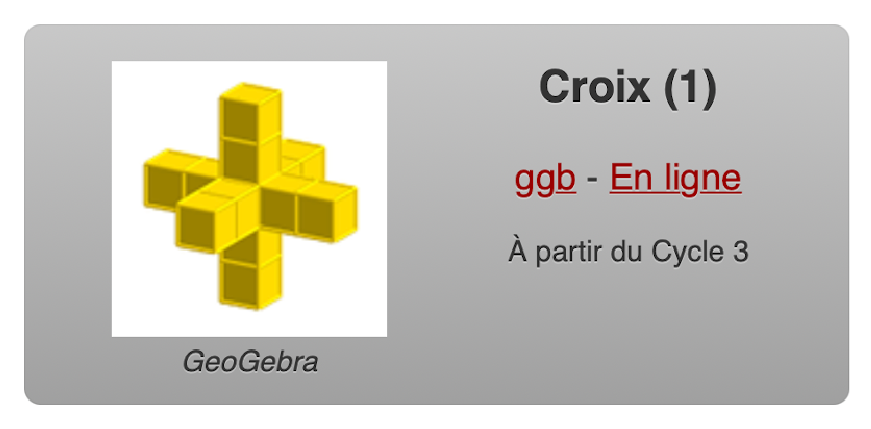
\includegraphics[width=7.5cm]{rubricamaths1} & 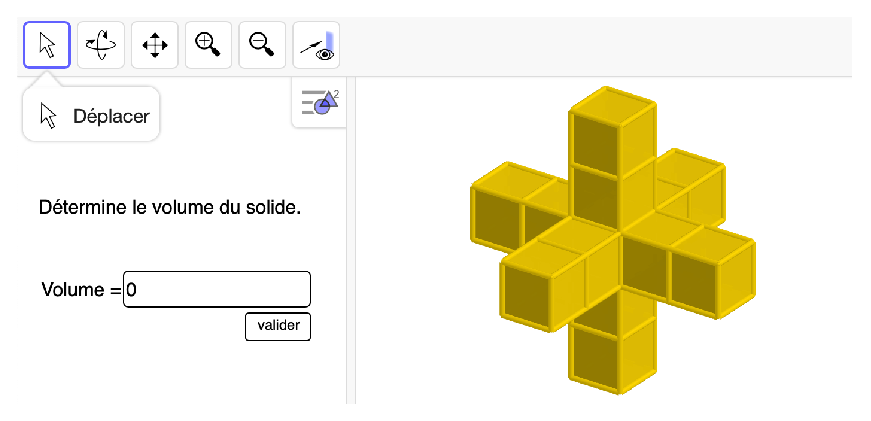
\includegraphics[width=7.5cm]{rubricamaths2} \\
   \end{tabular}
   
   \vfill
   
   \partie[Partie 2 - Restitution des résultats]
   Pour chaque solide, écrire le résultat (juste) que vous avez obtenu sur le site Internet dans le tableau suivant. \\
   Vous avez le droit à autant d'essais que vous le souhaitez.
   \begin{center}
      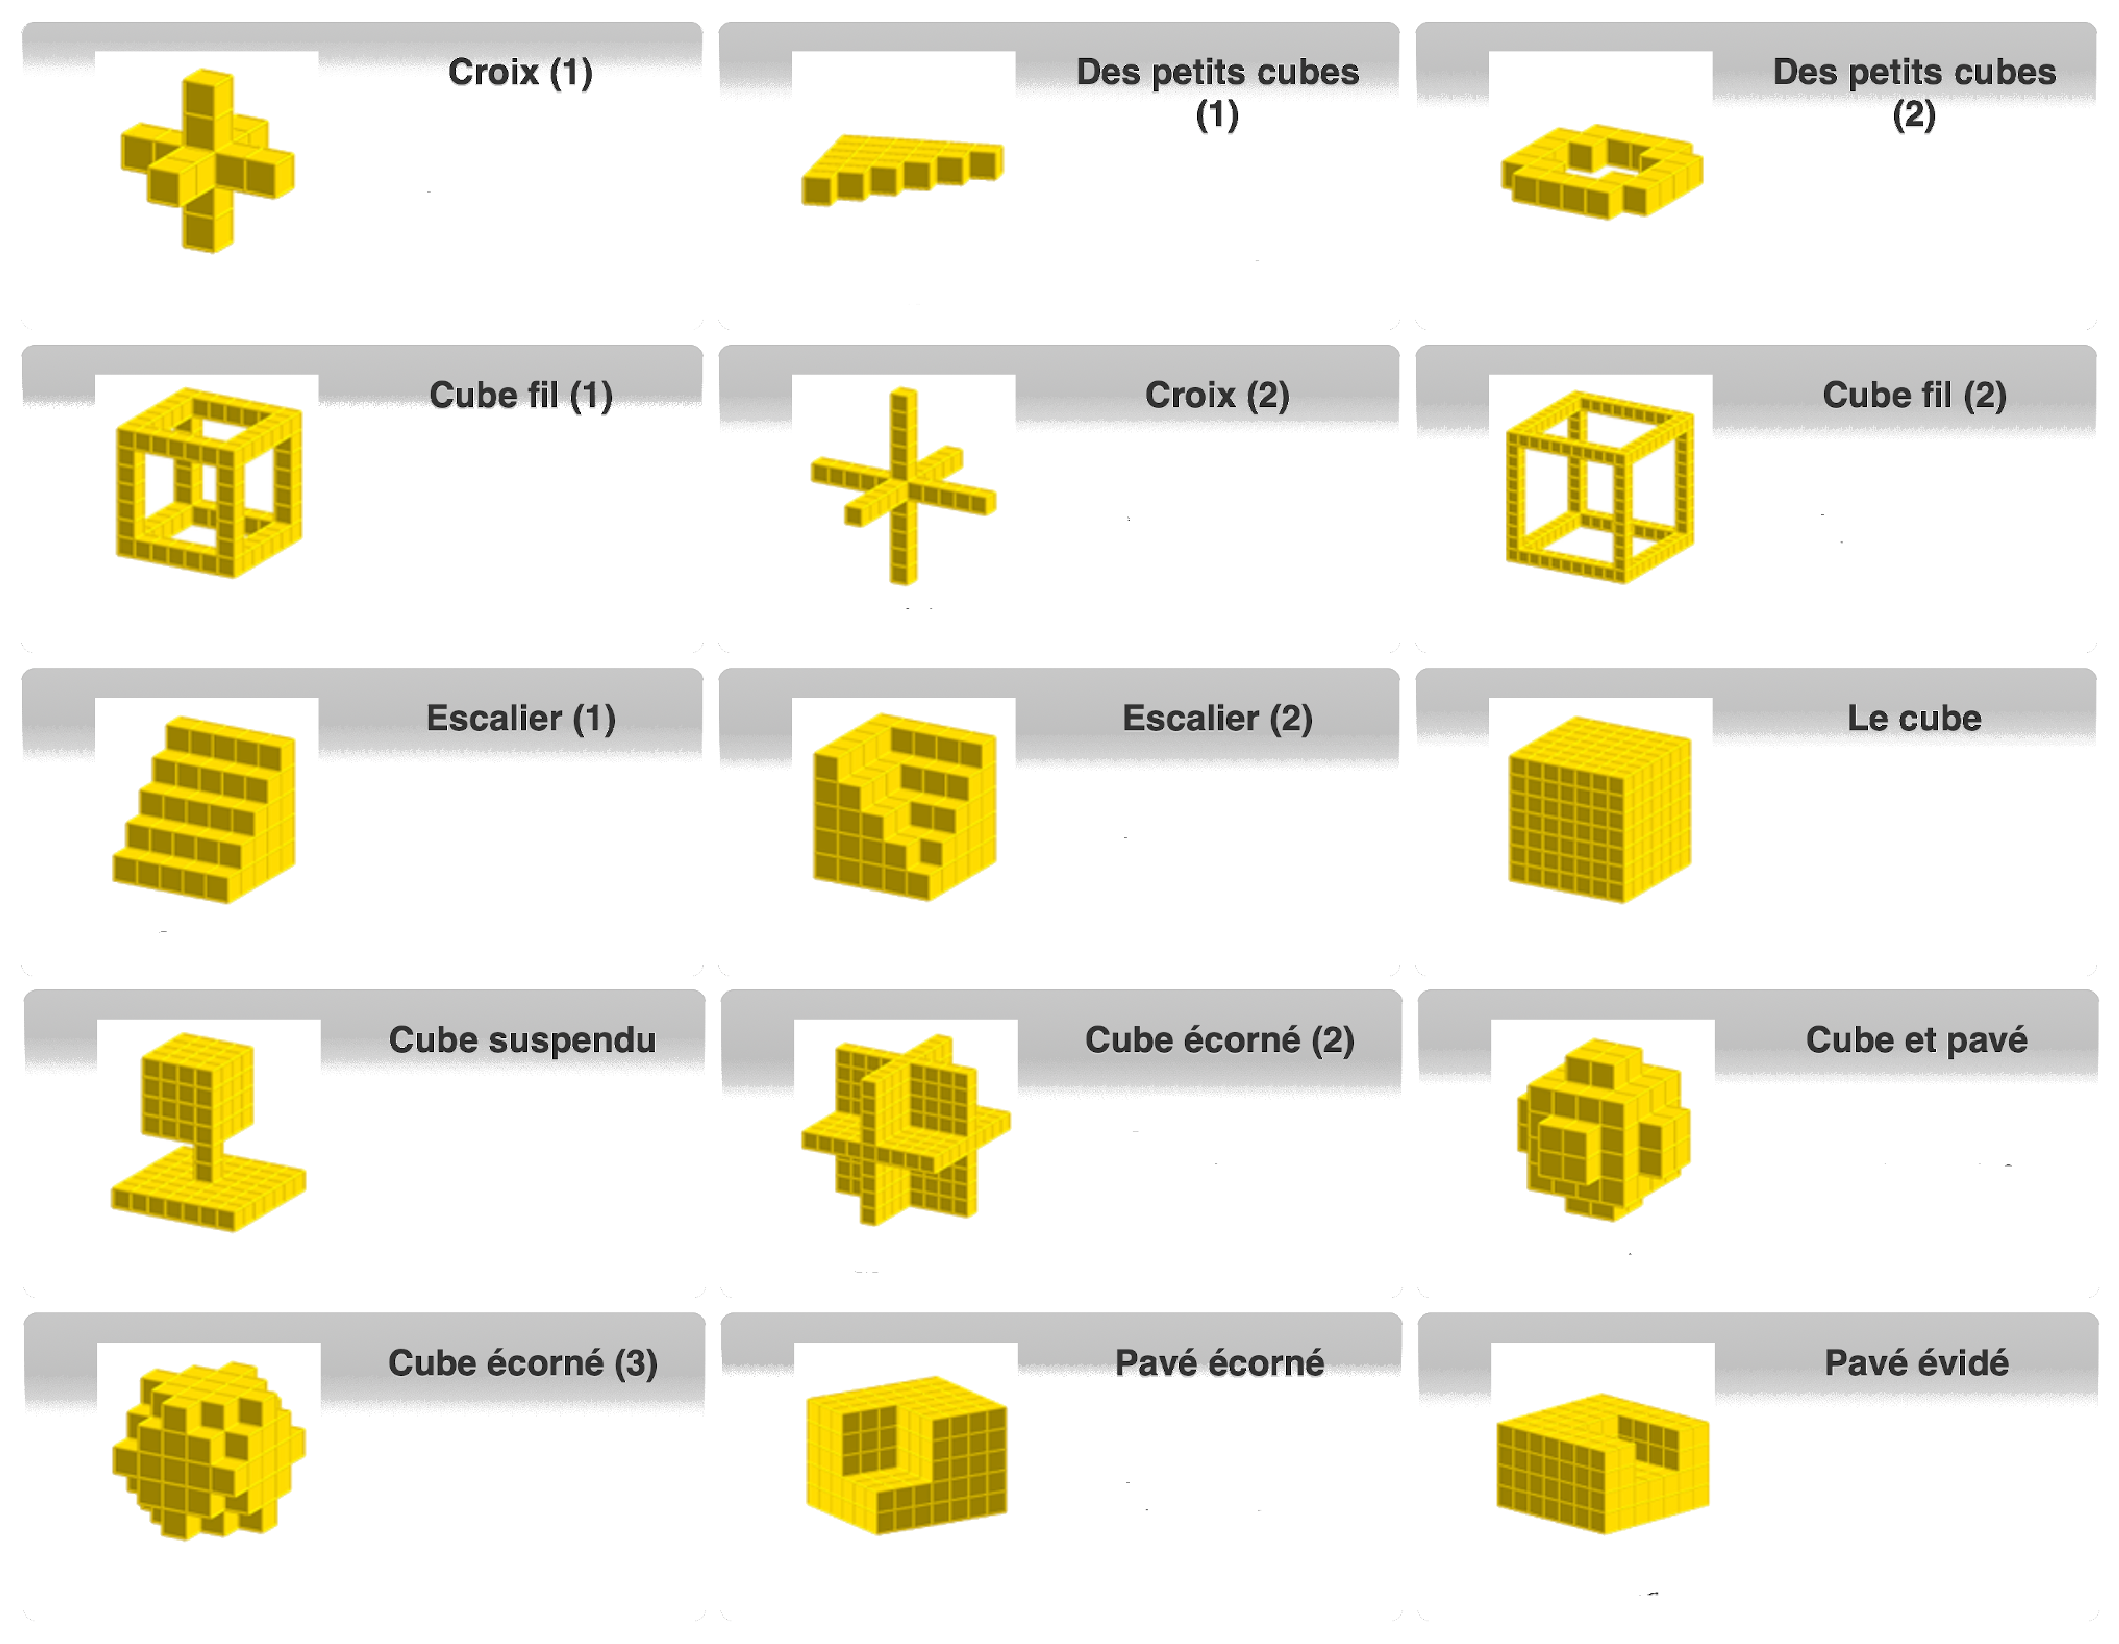
\includegraphics[width=16cm]{rubricamaths3}
   \end{center}
